\documentclass{standalone}
\usepackage{xparse}
\usepackage{tikz}
\usetikzlibrary{arrows}
\usetikzlibrary{calc}
\tikzset{%
  point/.style={circle,inner sep=1.25pt,minimum size=1.25pt,draw,fill=#1},
  point/.default=red
}
\definecolor{c0}{rgb}{0.2,0.4,0.67}
\definecolor{c1}{rgb}{0.67,0.4,0.12}
\definecolor{c2}{rgb}{0.53,0.6,0.13}
\definecolor{c3}{rgb}{0.53,0.53,0.4}
\NewDocumentCommand\witness{mmmO{c2}}{%
  \node[point=#4] (w0) at (#1) {};
  \node[point=#4] (w1) at (#2) {};
  \node[point=#4] (w2) at (#3) {};
  \draw[#4] (w0)--(w1)--(w2);
}
\NewDocumentCommand\elipricArc{mm}{
  \draw[c1,thick] ($(0, 0) + (0:#1 cm and #2 cm)$(P) arc (0:90:#1 cm and #2 cm);
}
\def\myWitness{\witness{0,0}{\x,\y}{\dc,0}}
\begin{document}
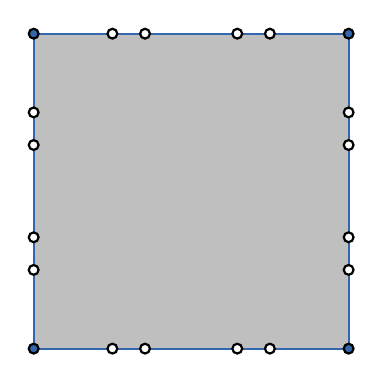
\begin{tikzpicture}[thick]
  % Boundary
  \coordinate (b0) at (-2,-2);
  \coordinate (b1) at (2,-2);
  \coordinate (b2) at (2,2);
  \coordinate (b3) at (-2,2);
  \filldraw[fill=lightgray,draw=c0] (b0) -- (b1) -- (b2) -- (b3) -- cycle;
  \node[point=c0] at (b0) {};
  \node[point=c0] at (b1) {};
  \node[point=c0] at (b2) {};
  \node[point=c0] at (b3) {};
  \begin{scope}[rotate=0,shift={(-2,-2)}]
    \elipricArc{1.4142}{1}
    \elipricArc{1}{1.4142}
    \node[point=white] at (0,1.4142) {};
    \node[point=white] at (1.4142,0) {};
    \node[point=white] at (0,1) {};
    \node[point=white] at (1,0) {};
  \end{scope}
  \begin{scope}[rotate=90,shift={(-2,-2)}]
    \elipricArc{1.4142}{1}
    \elipricArc{1}{1.4142}
    \node[point=white] at (0,1.4142) {};
    \node[point=white] at (1.4142,0) {};
    \node[point=white] at (0,1) {};
    \node[point=white] at (1,0) {};
  \end{scope}
  \begin{scope}[rotate=180,shift={(-2,-2)}]
    \elipricArc{1.4142}{1}
    \elipricArc{1}{1.4142}
    \node[point=white] at (0,1.4142) {};
    \node[point=white] at (1.4142,0) {};
    \node[point=white] at (0,1) {};
    \node[point=white] at (1,0) {};
  \end{scope}
  \begin{scope}[rotate=270,shift={(-2,-2)}]
    \elipricArc{1.4142}{1}
    \elipricArc{1}{1.4142}
    \node[point=white] at (0,1.4142) {};
    \node[point=white] at (1.4142,0) {};
    \node[point=white] at (0,1) {};
    \node[point=white] at (1,0) {};
  \end{scope}
  \pgfmathparse{2.4142}\let\dc\pgfmathresult
  \pgfmathparse{1}\let\x\pgfmathresult
  \pgfmathparse{0}\let\y\pgfmathresult
  \begin{scope}[rotate=-10,shift={(-1.694,-1.905)}]\myWitness\end{scope}
\end{tikzpicture}

\end{document}
